\documentclass[tikz, border=6pt]{standalone}
\IfFileExists{lmodern.sty}{\usepackage[T1]{fontenc}\usepackage{lmodern}}{}
\usepackage{amsmath,amssymb,bm}
\usetikzlibrary{arrows.meta, decorations.pathreplacing}
\definecolor{Blue}{HTML}{3A76D8}
\definecolor{Ink}{HTML}{1F2937}
\definecolor{cBACFF1}{HTML}{BACFF1}
\definecolor{cBCCCF1}{HTML}{BCCCF1}
\definecolor{cBDC9F0}{HTML}{BDC9F0}
\definecolor{cBFC6EF}{HTML}{BFC6EF}
\definecolor{cC0C3EE}{HTML}{C0C3EE}
\definecolor{cC2C0ED}{HTML}{C2C0ED}
\definecolor{cC3BDED}{HTML}{C3BDED}
\definecolor{cC5BAEC}{HTML}{C5BAEC}
\definecolor{cC6B7EB}{HTML}{C6B7EB}
\definecolor{cC8B4EA}{HTML}{C8B4EA}
\begin{document}
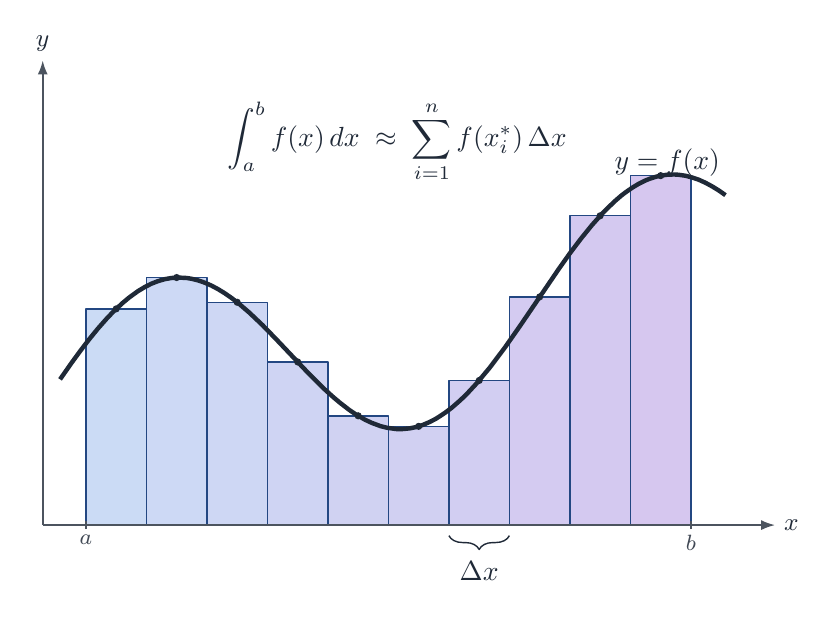
\begin{tikzpicture}[color=Ink, line width=0.5pt, >={Latex[length=5pt, width=3.6pt]}, line join=round]
  % axes ax1
  \begin{scope}
    \clip (0,0) rectangle (9,5.6);
    \filldraw[fill=cBACFF1, draw=Blue!60!black, line width=0.5pt, fill opacity=0.75] (0.549,0) --
        (1.317,0) -- (1.317,2.746) -- (0.549,2.746) -- cycle;
    \filldraw[fill=cBCCCF1, draw=Blue!60!black, line width=0.5pt, fill opacity=0.75] (1.317,0) --
        (2.085,0) -- (2.085,3.144) -- (1.317,3.144) -- cycle;
    \filldraw[fill=cBDC9F0, draw=Blue!60!black, line width=0.5pt, fill opacity=0.75] (2.085,0) --
        (2.854,0) -- (2.854,2.83) -- (2.085,2.83) -- cycle;
    \filldraw[fill=cBFC6EF, draw=Blue!60!black, line width=0.5pt, fill opacity=0.75] (2.854,0) --
        (3.622,0) -- (3.622,2.072) -- (2.854,2.072) -- cycle;
    \filldraw[fill=cC0C3EE, draw=Blue!60!black, line width=0.5pt, fill opacity=0.75] (3.622,0) --
        (4.39,0) -- (4.39,1.388) -- (3.622,1.388) -- cycle;
    \filldraw[fill=cC2C0ED, draw=Blue!60!black, line width=0.5pt, fill opacity=0.75] (4.39,0) --
        (5.159,0) -- (5.159,1.254) -- (4.39,1.254) -- cycle;
    \filldraw[fill=cC3BDED, draw=Blue!60!black, line width=0.5pt, fill opacity=0.75] (5.159,0) --
        (5.927,0) -- (5.927,1.837) -- (5.159,1.837) -- cycle;
    \filldraw[fill=cC5BAEC, draw=Blue!60!black, line width=0.5pt, fill opacity=0.75] (5.927,0) --
        (6.695,0) -- (6.695,2.898) -- (5.927,2.898) -- cycle;
    \filldraw[fill=cC6B7EB, draw=Blue!60!black, line width=0.5pt, fill opacity=0.75] (6.695,0) --
        (7.463,0) -- (7.463,3.928) -- (6.695,3.928) -- cycle;
    \filldraw[fill=cC8B4EA, draw=Blue!60!black, line width=0.5pt, fill opacity=0.75] (7.463,0) --
        (8.232,0) -- (8.232,4.438) -- (7.463,4.438) -- cycle;
    \draw[color=Ink, line width=1.6pt] (0.22,1.851) -- (0.361,2.053) -- (0.474,2.208) -- (0.587,2.356)
        -- (0.7,2.495) -- (0.813,2.623) -- (0.898,2.712) -- (1.011,2.818) -- (1.096,2.889) --
        (1.209,2.971) -- (1.294,3.022) -- (1.378,3.065) -- (1.463,3.098) -- (1.548,3.123) --
        (1.633,3.138) -- (1.718,3.144) -- (1.831,3.138) -- (1.887,3.129) -- (1.972,3.108) --
        (2.057,3.079) -- (2.142,3.042) -- (2.226,2.997) -- (2.311,2.945) -- (2.396,2.886) --
        (2.481,2.821) -- (2.622,2.7) -- (2.792,2.539) -- (2.961,2.365) -- (3.357,1.947) -- (3.583,1.722)
        -- (3.696,1.62) -- (3.781,1.549) -- (3.894,1.462) -- (3.979,1.405) -- (4.092,1.339) --
        (4.177,1.299) -- (4.29,1.257) -- (4.374,1.236) -- (4.488,1.22) -- (4.572,1.22) -- (4.657,1.228)
        -- (4.742,1.245) -- (4.827,1.272) -- (4.911,1.308) -- (4.996,1.352) -- (5.109,1.426) --
        (5.194,1.49) -- (5.307,1.589) -- (5.392,1.672) -- (5.505,1.794) -- (5.675,1.997) -- (5.873,2.26)
        -- (6.07,2.542) -- (6.551,3.249) -- (6.692,3.448) -- (6.834,3.636) -- (6.975,3.81) --
        (7.116,3.968) -- (7.257,4.106) -- (7.342,4.18) -- (7.399,4.224) -- (7.484,4.283) --
        (7.568,4.334) -- (7.653,4.376) -- (7.71,4.399) -- (7.795,4.426) -- (7.851,4.439) -- (7.936,4.45)
        -- (8.021,4.453) -- (8.077,4.449) -- (8.162,4.437) -- (8.247,4.415) -- (8.332,4.386) --
        (8.416,4.348) -- (8.501,4.302) -- (8.586,4.25) -- (8.671,4.19);
    \fill[Ink] (0.933,2.746) circle[radius=1.3pt];
    \fill[Ink] (1.701,3.144) circle[radius=1.3pt];
    \fill[Ink] (2.47,2.83) circle[radius=1.3pt];
    \fill[Ink] (3.238,2.072) circle[radius=1.3pt];
    \fill[Ink] (4.006,1.388) circle[radius=1.3pt];
    \fill[Ink] (4.774,1.254) circle[radius=1.3pt];
    \fill[Ink] (5.543,1.837) circle[radius=1.3pt];
    \fill[Ink] (6.311,2.898) circle[radius=1.3pt];
    \fill[Ink] (7.079,3.928) circle[radius=1.3pt];
    \fill[Ink] (7.848,4.438) circle[radius=1.3pt];
  \end{scope}
  \draw[->, Ink!80, line width=0.6pt] (0,0) -- (9.3,0);
  \draw[->, Ink!80, line width=0.6pt] (0,0) -- (0,5.9);
  \draw[Ink!80, line width=0.5pt] (0.549,-0.05) -- (0.549,0.05) (8.232,-0.05) -- (8.232,0.05);
  \node[anchor=north, font=\footnotesize, text=Ink!85, inner sep=2pt] (ax1-xt0) at (0.549,-0.05) {$a$};
  \node[anchor=north, font=\footnotesize, text=Ink!85, inner sep=2pt] (ax1-xt1) at (8.232,-0.05) {$b$};
  \node[anchor=south east] at (8.726,4.301) {$y = f(x)$};
  \node[anchor=west, font=\small, align=center, inner sep=3pt] at (9.3,0) {$x$};
  \node[anchor=south, font=\small, align=center, inner sep=3pt] at (0,5.9) {$y$};
  \draw[decorate, decoration={brace, amplitude=5pt, raise=2pt}] (5.9268,-0.0636) -- (5.1585,-0.0636)
      node[midway, auto, outer sep=8pt] {$\Delta x$};
  \node[anchor=north, inner sep=4pt] at (4.5,5.5364) {$\displaystyle\int_a^b f(x)\,dx \;\approx\; \sum_{i=1}^{n} f(x_i^*)\,\Delta x$};
\end{tikzpicture}
\end{document}
